% Berapa Kali Setengah Muat dalam Dua? — Pembagian Pecahan dengan TikZ
% Gunanto · pakgun.gezytech.web.id
% Siap kompilasi: pdflatex pembagian-pecahan.tex (butuh paket tikz dan amsmath)
\documentclass{article}
\usepackage[a4paper,margin=2cm]{geometry}
\usepackage{amsmath}
\usepackage{tikz}
\usepackage{xcolor}

\definecolor{aksen}{HTML}{F7B538}
\definecolor{abu}{gray}{0.6}

\begin{document}

\section*{Gambar 1: Model Pita --- $2 : \frac{1}{2}$}

Pita sepanjang 2 satuan dipotong tiap $\frac{1}{2}$: ada empat potong.

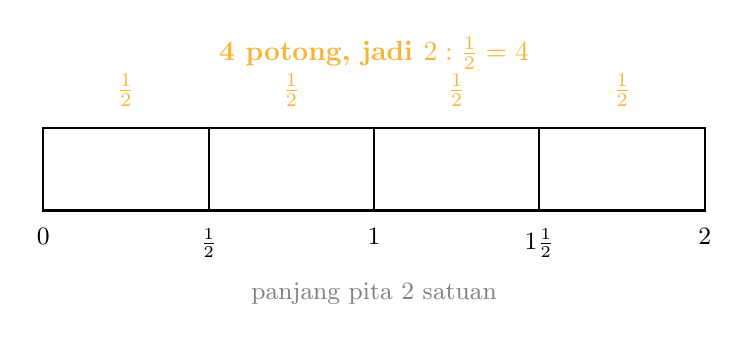
\begin{tikzpicture}[line cap=round, x=1.05cm, y=1.05cm]
  \draw[thick] (0,0) rectangle (8,1);
  \foreach \x in {2,4,6} \draw[thick] (\x,0) -- (\x,1);
  \foreach \x in {1,3,5,7} \node[above=4pt, text=aksen] at (\x,1) {$\frac{1}{2}$};
  \foreach \x/\t in {0/$0$,2/$\frac{1}{2}$,4/$1$,6/$1\frac{1}{2}$,8/$2$}
     \node[below=3pt, font=\small] at (\x,0) {\t};
  \node[text=aksen, font=\bfseries] at (4,1.9) {4 potong, jadi $2 : \frac{1}{2} = 4$};
  \node[text=gray, font=\small] at (4,-1.0) {panjang pita 2 satuan};
\end{tikzpicture}

\section*{Gambar 2: Model Persegi --- $\frac{3}{4} : \frac{1}{6}$}

Garis kuning mendatar membagi persegi menjadi empat baris (perempat);
garis abu tegak membaginya menjadi enam kolom (perenam).
Keduanya bertemu membentuk $4 \times 6 = 24$ kotak kecil, tiap kotak $\frac{1}{24}$.

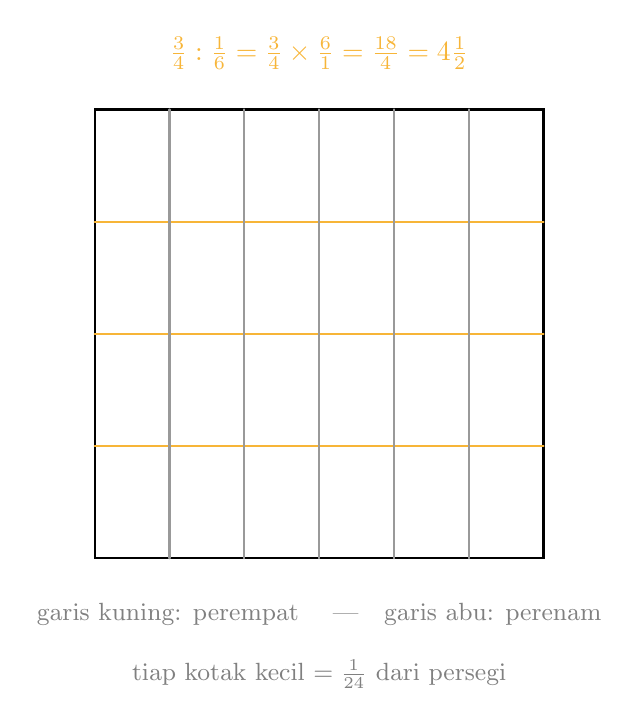
\begin{tikzpicture}[line cap=round, x=0.95cm, y=0.95cm]
  \draw[thick] (0,0) rectangle (6,6);
  \foreach \y in {1.5,3,4.5} \draw[aksen, thick] (0,\y) -- (6,\y);
  \foreach \x in {1,2,3,4,5} \draw[abu, thick] (\x,0) -- (\x,6);
  \node[text=aksen, font=\bfseries] at (3,6.75)
    {$\frac{3}{4} : \frac{1}{6} = \frac{3}{4} \times \frac{6}{1} = \frac{18}{4} = 4\frac{1}{2}$};
  \node[text=gray, font=\small, align=center] at (3,-0.75)
    {garis kuning: perempat \quad|\quad garis abu: perenam};
  \node[text=gray, font=\small, align=center] at (3,-1.55)
    {tiap kotak kecil $=\frac{1}{24}$ dari persegi};
\end{tikzpicture}

\end{document}
